\documentclass{exam}
\usepackage[utf8]{inputenc}
\usepackage{lmodern}
\usepackage{microtype}

% \usepackage[parfill]{parskip}
\usepackage[dvipsnames]{xcolor}
\usepackage{amsmath}
\usepackage{amsfonts}
\usepackage{amsthm}
\usepackage{siunitx}
\DeclareSIUnit\year{yr}
\DeclareSIUnit\foot{ft}
\DeclareSIUnit\litre{\liter}

\usepackage{skull}

\usepackage{pgfplots}
\usepgfplotslibrary{polar}
\pgfplotsset{compat=1.11}
\usepgfplotslibrary{statistics}
\usepackage{graphicx}
\usepackage{sidecap}
\sidecaptionvpos{figure}{c}
\usepackage{float}
\usepackage{gensymb}
\usepackage{tkz-euclide}
\usetkzobj{all}
\usepackage{commath}
\usepackage{hyperref}
\usepackage{enumitem}
\usepackage{wasysym}
\usepackage{multicol}
\usepackage{mathtools}
\usepackage{tcolorbox}
\usepackage{tabularx}
\usepackage[version=4]{mhchem}
\usepackage{changepage}
\usepackage{listings}
\lstset{basicstyle=\ttfamily\linespread{0.8}\small}

\renewcommand*{\thefootnote}{\fnsymbol{footnote}}

\newtheorem*{thm}{Theorem}
\newtheorem*{iden}{Identity}
\newtheorem*{lemma}{Lemma}
\newtheorem{obs}{Observation}
\theoremstyle{definition}
\newtheorem*{defn}{Definition}
\newtheorem*{ex}{Example}
\newtheorem{con}{Construction}
\newtheorem*{alg}{Algorithm}

\newtheoremstyle{break}
  {\topsep}{\topsep}%
  {\itshape}{}%
  {\bfseries}{}%
  {\newline}{}%
\theoremstyle{break}
\newtheorem*{bthm}{Theorem}

% russian integral
\usepackage{scalerel}
\DeclareMathOperator*{\rint}{\scalerel*{\rotatebox{17}{$\!\int\!$}}{\int}}

% \DeclareMathOperator*{\rint}{\int}

\pgfplotsset{vasymptote/.style={
    before end axis/.append code={
        \draw[densely dashed] ({rel axis cs:0,0} -| {axis cs:#1,0})
        -- ({rel axis cs:0,1} -| {axis cs:#1,0});
    }
}}

% \pointsinrightmargin
\boxedpoints
\pointname{}

\newcommand{\questioA}{\question[\texttt{\textbf{\color{Cerulean} A}}]}
\newcommand{\questioM}{\question[\texttt{\textbf{\color{PineGreen} M}}]}
\newcommand{\questioE}{\question[\texttt{\textbf{\color{WildStrawberry} E}}]}
\newcommand{\questioS}{\question[\texttt{\textbf{\color{Goldenrod} S}}]}
\newcommand{\questioO}{\question[\texttt{\textbf{\color{BurntOrange} O}}]}

\newcommand{\parA}{\part[\texttt{\textbf{\color{Cerulean} A}}]}
\newcommand{\parM}{\part[\texttt{\textbf{\color{PineGreen} M}}]}
\newcommand{\parE}{\part[\texttt{\textbf{\color{WildStrawberry} E}}]}
\newcommand{\parS}{\part[\texttt{\textbf{\color{Goldenrod} S}}]}
\newcommand{\parO}{\part[\texttt{\textbf{\color{BurntOrange} O}}]}

\newcommand{\subparA}{\subpart[\texttt{\textbf{\color{Cerulean} A}}]}
\newcommand{\subparM}{\subpart[\texttt{\textbf{\color{PineGreen} M}}]}
\newcommand{\subparE}{\subpart[\texttt{\textbf{\color{WildStrawberry} E}}]}
\newcommand{\subparS}{\subpart[\texttt{\textbf{\color{Goldenrod} S}}]}
\newcommand{\subparO}{\subpart[\texttt{\textbf{\color{BurntOrange} O}}]}

\newcommand{\mainHeader}[2]{\section*{NCEA Level 2 Mathematics\\#1. #2}}
\newcommand{\mainHeaderHw}[2]{\section*{NCEA Level 2 Mathematics (Homework)\\#1. #2}}
\newcommand{\seealso}[1]{\begin{center}\emph{See also #1.}\end{center}}
\newcommand{\drills}[1]{\begin{center}\emph{Drill problems: #1.}\end{center}}
\newcommand{\basedon}[1]{\begin{center}\emph{Notes largely based on #1.}\end{center}}


\begin{document}

\mainHeaderHw{23}{Probability Distributions}
\subsection*{Reading}
\begin{center}
\begin{tcolorbox}[width=0.8\textwidth,colback={white},title={\textbf{Go and watch...}},colbacktitle=black,coltitle=white]
  \textcolor{black}{\url{https://www.youtube.com/watch?v=UCmPmkHqHXk}}
\end{tcolorbox}
\end{center}

\begin{center}
  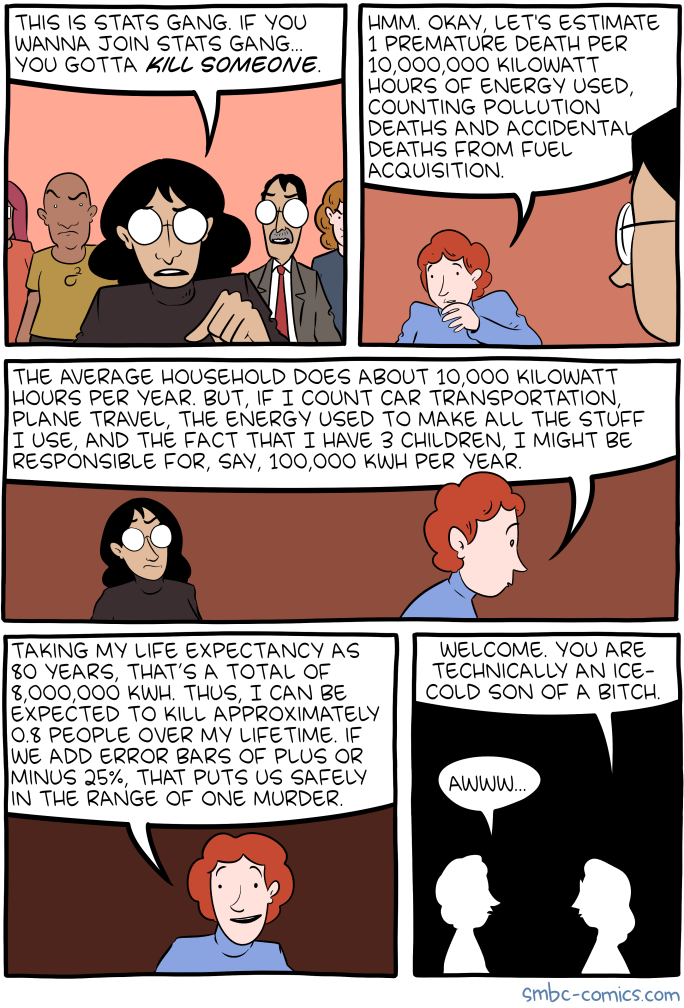
\includegraphics[width=0.6\textwidth]{killerstats}\\
  \small{\url{https://www.smbc-comics.com/comic/stats-gang}}
\end{center}


\subsection*{Questions}
\begin{questions}
  \item How are probability distributions related to the kind of data analysis we began probability with? Discuss. (Write
        around half a page, and do some research.)
  \item In 2017, one of the Census at School questions asked for the amount of water, in millilitres, drunk in the last day.
        The following graphs and statistical information shows the data for this question for students who drove to school, and
        for students who walked.
        \begin{center}
          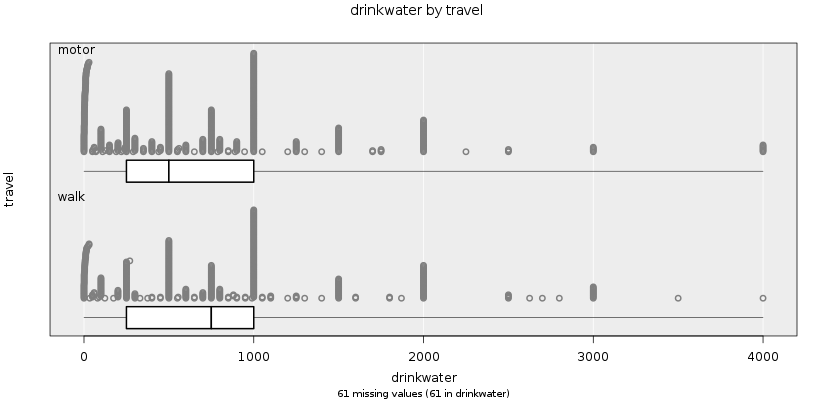
\includegraphics[width=0.9\textwidth]{drinktravel1}
        \end{center}
\begin{verbatim}
==========================================================================
                           iNZight Summary
--------------------------------------------------------------------------
        Primary variable of interest: travel (categorical)
                  Secondary variable: drinkwater (numeric)

        Total number of observations: 1000
   Number omitted due to missingness: 61 (61 in drinkwater)
   Total number of observations used: 939
==========================================================================

Summary of drinkwater by travel:
--------------------------------

           Min   25%   Median    75%    Max    Mean      SD   Sample Size
   motor     0   250      500   1000   4000   728.5   707.1           530
    walk     0   250      750   1000   4000   825.9   733.1           409


==========================================================================
\end{verbatim}
    \begin{parts}
      \part Compare and contrast the shapes of the statistics for the two groups.
      \part Is there any meaningful difference between the volume of water drunk in the last day between the two groups?
      \part Calculate the probability that a randomly chosen person from each group drank more than 800 mililitres in the
            last day. What is the relative risk --- is a walker more likely to have drunk more than 800 mililitres compared
            to a motorist?
      \part Suppose that at a particular school the mean value for water drunk in the last day (over all students) was
            \SI{712}{\milli\litre}. The survey also shows that only 10\% of students drank less than \SI{400}{\milli\litre}.
        \begin{subparts}
          \subpart What is the standard deviation of the sample in this case?
          \subpart What is the minimum amount of water for a student to have drunk in the last day in order to be
                   in the top 5\% of water drinkers, at this school?
        \end{subparts}
    \end{parts}
\end{questions}

\end{document}
